\documentclass{article}
\usepackage{amsmath,amssymb,amsthm}
\usepackage{geometry}
\usepackage{hyperref} % Added for clickable citations and URL
\usepackage{graphicx} % For benchmark figure
\geometry{margin=1in}
% === Theorem-like environments ===
\newtheorem{definition}{Definition}
\newtheorem{theorem}{Theorem}
\newtheorem{remark}{Remark}
\begin{document}
\begin{center}
 {\fontsize{18}{20}\selectfont\bfseries Radial Dual Lattice Graphs via Admissible Hyperspherical Inversion: From Eisenstein Integers (2D) to Hurwitz Quaternions (4D) to the E8 Lattice (8D)}\\[1.2em]
Nathan O. Schmidt$^{1}$, Klee Irwin$^{2}$, and Natasha Urakhchina$^{2}$ \\[0.6em]
\textit{$^{1}$Cold Hammer Research \& Development LLC, Eagle, Idaho, USA} \\[0.1em]
\texttt{nate.o.schmidt@coldhammer.net}$^{1}$ \\[0.4em]
\textit{$^{2}$Quantum Gravity Research, Topanga, California, USA} \\[0.1em]
\texttt{klee@quantumgravityresearch.org}$^{2}$, \texttt{natasha@quantumgravityresearch.org}$^{2}$ \\[0.6em]
March 3, 2026
\end{center}
\begin{abstract}
We introduce \emph{radial dual lattice graphs} constructed via admissible hyperspherical inversion on the underlying nearest-neighbor lattice graphs. Beginning with the Eisenstein integers in 2D, we define an exact bijective duality between inner and outer vertex zones that is preserved under the graph structure. This construction bootstraps recursively to the Hurwitz quaternion lattice graph in 4D and the E8 lattice graph in 8D. At each dimension the inversion map induces a graph isomorphism that preserves adjacency, norms, and symmetry groups, yielding a fully discrete and reversible combinatorial self-duality between the outer- and inner-zone subgraphs of the radial dual graphs. In particular, the 8D radial dual supplies Cycle Clock Theory with an exact radial-folding operator that maps arbitrarily large-norm cycle clocks on the E8 lattice to compact inner-zone equivalents in the rational extension, thereby reducing computational complexity in the simulation and enumeration of quasicrystalline dynamics while preserving all combinatorial invariants. With a direct realization via the Cayley integers (integral octonions) in 8D, the framework further aligns with octonion-based models in quasicrystalline quantum gravity \cite{Dixon1994,Furey2016}. A complementary linear folding operator, given by the Moxness E8-to-H4 matrix \(H_{4\mathrm{fold}}\), maps the 8D radial dual directly onto the 600-cell geometry and its scaled copy \(\mathrm{H}_4\Phi\), enabling dimension reduction while preserving all algebraic invariants and further enhancing computational efficiency in Cycle Clock Theory applications. The framework is purely algebraic and geometric, operating on rational extensions of the underlying lattices and requiring no approximations or continuous relaxations. Additionally, the radial dual provides an exact algebraic tool for the shelling and scaling analyses in Cycle Clock Theory (Chapter 5 of the textbook), enabling compact inner-zone computations of shell multiplicities, orientation statistics, and number-theoretic decompositions while preserving all invariants.
\end{abstract}
% Note: This is merely a preliminary draft proof-of-concept.
\begin{remark}
This work generalizes the Tri-Quarter Framework \cite{Schmidt2025} from 2D to 4D and 8D while preserving its exact discrete and rational nature.
\end{remark}
\section{Introduction}
This framework operates on rational extensions of the underlying exceptional lattices, which are forced by the geometry of maximally dense sphere packings in the only dimensions (1, 2, 4, 8) that admit normed division algebras---a rigid construction that fundamentally terminates at 8D due to the Hopf invariant one theorem \cite{Adams1960}.
\section{2D Eisenstein Lattice Graph: Tri-Quarter Radial Dual}
Let \(\omega = e^{2\pi i / 3} = -\frac{1}{2} + i \frac{\sqrt{3}}{2}\) be a primitive cube root of unity. The Eisenstein integers form the ring
\[
\mathbb{Z}[\omega] = \{ m + n\omega \mid m,n \in \mathbb{Z} \}.
\]
The associated lattice \(L^{2D} \subset \mathbb{C} \cong \mathbb{R}^2\) is given by the explicit embedding
\[
\mathbf{z} = m + n\omega = \Bigl(m - \frac{n}{2}\Bigr) + i \frac{n\sqrt{3}}{2},
\]
with squared Euclidean norm
\[
N(\mathbf{z}) = m^2 - mn + n^2 \in \mathbb{N}_0.
\]
\textbf{Explanation of the norm}: This quadratic form is precisely the squared Euclidean distance \(|\mathbf{z}|^2\) in the plane. It is positive definite, integer-valued on the lattice, and generates perfect hexagonal shells of radius \(\sqrt{k}\) for admissible integers \(k\).
\begin{definition}
The \emph{underlying lattice graph} \(\Lambda^{2D}\) is the infinite undirected graph with
\begin{itemize}
  \item vertices: all points of \(L^{2D}\),
  \item edges: pairs \(\{\mathbf{z}, \mathbf{w}\}\) such that \(N(\mathbf{z} - \mathbf{w}) = 1\) (nearest-neighbor minimal vectors).
\end{itemize}
\end{definition}
\begin{remark}
\(\Lambda^{2D}\) is the infinite triangular (hexagonal) grid graph. Every vertex has degree exactly 6, reflecting the six nearest neighbors at 60° intervals. The full symmetry group is the dihedral group \(D_6\) of order 12, generated by 60° rotations and reflections, which acts transitively on the vertices and preserves the graph structure.
\end{remark}
\subsection{Admissible Inversion Radius}
A radius \(r > 0\) is \emph{admissible} if \(r^2 = N(\mathbf{z})\) for some nonzero \(\mathbf{z} \in L^{2D}\). For the canonical choice \(r=1\) (\(N=1\)), the boundary shell consists of exactly six vertices forming a regular hexagon centered at the origin. Admissibility guarantees that the boundary is a discrete, symmetry-invariant set with no fractional radii, ensuring the inversion map sends lattice points to points in the rational extension.
\subsection{Zone Partitioning}
Fix an admissible \(r > 0\). Partition the vertex set of \(\Lambda^{2D} \setminus \{0\}\) into three disjoint subsets:
\begin{itemize}
  \item Outer zone (vertices): \(\Lambda_{+,r}^{2D} = \{ \mathbf{z} \in L^{2D} \mid N(\mathbf{z}) > r^2 \}\),
  \item Boundary zone (vertices): \(\Lambda_{T,r}^{2D} = \{ \mathbf{z} \in L^{2D} \mid N(\mathbf{z}) = r^2 \}\),
  \item Inner zone (vertices): \(\Lambda_{-,r}^{2D} = \iota_r(\Lambda_{+,r}^{2D})\), consisting of points in \(\mathbb{Q}(\omega)\) obtained by inversion (generally with rational coefficients in the Eisenstein basis).
\end{itemize}
The full radial dual lattice graph \(\Lambda_r^{2D}\) has vertex set
\[
V(\Lambda_r^{2D}) = \Lambda_{-,r}^{2D} \cup \Lambda_{T,r}^{2D} \cup \Lambda_{+,r}^{2D},
\]
where the inner-zone points lie in the rational vector space spanned by the lattice (not necessarily in \(L^{2D}\)).
\textbf{Intuitive remark}: The three zones create a “tri-quarter” partition of the punctured plane. The outer zone contains all “far-away” lattice points, the boundary is the fixed shell, and the inner zone is the exact algebraic reflection of the outer zone through the circle of radius \(r\).
\subsection{Circle Inversion Map}
Define the inversion on nonzero lattice points by
\[
\iota_r(\mathbf{z}) = \frac{r^2 \, \mathbf{z}}{N(\mathbf{z})}.
\]
This map satisfies the following properties (verified algebraically in sequence):
\begin{enumerate}
  \item \textbf{Involution}: \(\iota_r(\iota_r(\mathbf{z})) = \mathbf{z}\).
  \item \textbf{Boundary fixed set}: If \(N(\mathbf{z}) = r^2\) then \(\iota_r(\mathbf{z}) = \mathbf{z}\).
  \item \textbf{Zone swap}: \(\iota_r(\Lambda_{+,r}^{2D}) = \Lambda_{-,r}^{2D}\) and vice versa.
  \item \textbf{Angular preservation}: \(\arg(\iota_r(\mathbf{z})) = \arg(\mathbf{z})\); each point and its dual lie on the same radial ray from the origin.
  \item \textbf{Norm relation}: \(N(\iota_r(\mathbf{z})) = r^4 / N(\mathbf{z})\).
\end{enumerate}
\begin{remark}
Geometrically, \(\iota_r\) rescales every point radially through the circle of radius \(r\): points far outside are mapped close to the origin along the same radial ray, and vice versa. Because the map is a positive scalar multiple of the identity on each ray, it is conformal and angle-preserving, respecting the 60° angular structure of the triangular lattice. This is the key geometric intuition that makes the construction work across dimensions.
\end{remark}
\begin{remark}
Although \(\iota_r\) does not in general map \(L^{2D}\) into itself, it produces a countably infinite discrete set of points in \(\mathbb{Q}(\omega)\) that is in bijective correspondence with the outer zone. This is precisely the construction used in the Tri-Quarter Framework \cite{Schmidt2025}, where the inner zone forms a dual point cloud accumulating at the origin.
\end{remark}
\subsection{Graph Construction and Duality}
The edge set \(E(\Lambda_r^{2D})\) of the radial dual lattice graph is defined in three parts (nested by zone):
\begin{itemize}
  \item \textbf{Outer-zone edges}: all nearest-neighbor edges of \(\Lambda^{2D}\) with both endpoints in \(\Lambda_{+,r}^{2D}\),
  \item \textbf{Inner-zone edges}: the images \(\{\iota_r(\mathbf{z}), \iota_r(\mathbf{w})\}\) of every outer-zone edge \(\{\mathbf{z}, \mathbf{w}\}\),
  \item \textbf{Boundary-crossing edges}: for each pair consisting of a boundary vertex \(\mathbf{z} \in \Lambda_{T,r}^{2D}\) and an outer vertex \(\mathbf{w} \in \Lambda_{+,r}^{2D}\) that are adjacent in \(\Lambda^{2D}\), add the edge \(\{\mathbf{z}, \iota_r(\mathbf{w})\}\).
\end{itemize}
\begin{theorem}[2D Bijective Radial Graph Duality]
For any admissible \(r\), the restriction of \(\iota_r\) induces a graph isomorphism
\[
\iota_r \colon (\Lambda_{+,r}^{2D}, E(\Lambda_r^{2D})|_{\Lambda_{+,r}^{2D}}) \;\to\; (\Lambda_{-,r}^{2D}, E(\Lambda_r^{2D})|_{\Lambda_{-,r}^{2D}}).
\]
\end{theorem}
\begin{proof}
The map \(\iota_r\) is an algebraic involution (\(\iota_r \circ \iota_r = \mathrm{id}\)) that swaps the outer and inner zones bijectively, as \(N(\iota_r(\mathbf{z})) = r^4 / N(\mathbf{z})\) and admissibility of \(r\) ensures all points remain in the rational extension \(\mathbb{Q}(\omega)\). By construction of the edge set, every outer-zone nearest-neighbor edge \(\{\mathbf{z}, \mathbf{w}\}\) (both in \(\Lambda_{+,r}^{2D}\)) maps directly to the inner-zone edge \(\{\iota_r(\mathbf{z}), \iota_r(\mathbf{w})\}\). Boundary-crossing edges \(\{\mathbf{z}, \mathbf{w}\}\) (with \(\mathbf{z} \in \Lambda_{T,r}^{2D}\), \(\mathbf{w} \in \Lambda_{+,r}^{2D}\)) are mirrored by the addition of the symmetric edge on the inner side via the involution property and fixed boundary. Thus adjacency is preserved exactly. The dihedral symmetry group \(D_6\) commutes with \(\iota_r\) because circle inversion through the origin-centered admissible shell is conformal and angle-preserving, and the lattice is \(D_6\)-invariant. Therefore \(\iota_r\) is a graph isomorphism between the induced subgraphs.
\end{proof}
% TODO: Insert figure of the Eisenstein triangular lattice graph (hexagonal grid with labeled zones)
\section{Bootstrapping to 4D: Hurwitz Quaternion Lattice Graph Radial Dual}
\subsection{Hurwitz Quaternion Lattice Graph}
The Hurwitz integers \(\mathbb{H}\) consist of all quaternions
\[
q = a + bi + cj + dk, \quad a,b,c,d \in \tfrac{1}{2}\mathbb{Z},
\]
such that \(a,b,c,d\) are either all integers or all half-integers (\(a+b+c+d \in \mathbb{Z}\)). This is the standard maximal order in the quaternion algebra.\cite{ConwaySmith2003} The lattice \(L^{4D} \subset \mathbb{R}^4\) carries the norm \(N(q) = a^2 + b^2 + c^2 + d^2\), which equals the squared Euclidean length in 4-space.
The underlying lattice graph \(\Lambda^{4D}\) has vertices \(L^{4D}\) and edges between points at minimal positive norm distance 1. Each vertex has degree 24, corresponding to the 24 units of \(\mathbb{H}\).
\subsection{Admissible Inversion Radius in 4D}
Choose admissible \(r > 0\) with \(r^2 = N(q)\) for some \(0 \neq q \in \mathbb{H}\) (e.g., \(r=1\) yields the 24 vertices of the regular 24-cell, a highly symmetric polytope in 4D \cite{Coxeter1973}). Admissibility again ensures discrete shells invariant under the full symmetry group of \(\Lambda^{4D}\).
\subsection{Zone Partitioning in 4D}
Partition the vertices of \(\Lambda^{4D} \setminus \{0\}\) exactly as in 2D:
\begin{itemize}
  \item Outer: \(\Lambda_{+,r}^{4D} = \{ q \in L^{4D} \mid N(q) > r^2 \}\),
  \item Boundary: \(\Lambda_{T,r}^{4D} = \{ q \in L^{4D} \mid N(q) = r^2 \}\),
  \item Inner: \(\Lambda_{-,r}^{4D} = \iota_r(\Lambda_{+,r}^{4D})\), consisting of points in the rational extension \(\mathbb{Q} \otimes_{\mathbb{Z}} \mathbb{H}\).
\end{itemize}
The radial dual lattice graph is \(\Lambda_r^{4D}\) with vertex set \(\Lambda_{-,r}^{4D} \cup \Lambda_{T,r}^{4D} \cup \Lambda_{+,r}^{4D}\).
\subsection{Hyperspherical Inversion in 4D}
\[
\iota_r(q) = \frac{r^2 \, q}{N(q)}.
\]
The five algebraic properties listed in the 2D case hold verbatim (replacing \(\mathbf{z}\) by \(q\)), now acting on the 3-sphere \(S^3\).
\begin{remark}
The map reflects vertices through the hypersphere of radius \(r\) in 4-space, exactly mirroring the 2D circle inversion. In higher dimensions the geometric intuition is the same: distant points are pulled inside and vice versa, while the rich \(SU(2) \times SU(2)\) symmetry of the 24-cell is preserved.
\end{remark}
\subsection{Bootstrapping Construction (2D \(\to\) 4D)}
The 4D radial dual lattice graph is constructed from the 2D pair via the following explicit steps:
\begin{enumerate}
  \item Select a 2D dual pair \((z_+, z_-) \in \Lambda_{+,r}^{2D} \times \Lambda_{-,r}^{2D}\) with \(z_- = \iota_r(z_+)\).
  \item Embed orthogonally in the quaternion basis:
        \[
        q = z_+ + z_- \, j.
        \]
  \item Form the quaternion \(q = z_+ + \iota_r(z_+) \, j\) (or any orthogonal embedding in the \(\{1,i,j,k\}\) basis). The resulting point lies in a rational extension of \(\mathbb{H}\).
  \item The set of all such \(q\) (together with their images under \(\iota_r\)) defines the vertex set of the 4D radial dual graph \(\Lambda_r^{4D}\); edges are inherited via the embedding and the 2D edge-mirroring rule.
\end{enumerate}
\textbf{Why this works}: The orthogonal embedding preserves the norm additively and commutes with radial scaling, so the 4D inversion \(\iota_r(q)\) is the image of the 2D inversion applied componentwise. The resulting inner-zone points lie in \(\mathbb{Q} \otimes_{\mathbb{Z}} \mathbb{H}\) and form a dual structure exactly analogous to the 2D case. The parity condition of Hurwitz integers is not required for the dual graph; only the combinatorial isomorphism is inherited.
\begin{theorem}[4D Bijective Radial Graph Duality]
\(\iota_r\) induces a graph isomorphism between the outer- and inner-zone induced subgraphs of \(\Lambda_r^{4D}\), preserving adjacency via edge mirroring and the integer-valued quadratic form on the outer zone. The symmetry group extends to an order-48 group \(\mathbb{T}_{48}\) (binary tetrahedral group extended by inversion).
\end{theorem}
\begin{proof}
The orthogonal embedding \(q = z_+ + \iota_r(z_+) j\) is isometric: \(N(q) = N(z_+) + N(\iota_r(z_+))\) by orthogonality of the quaternion basis. Componentwise application of the 2D isomorphism (Theorem above) yields a bijection between outer and inner 4D zones. Edge mirroring in 4D follows directly from the 2D rule because radial scaling and the embedding commute with \(\iota_r\). The gluing condition for Hurwitz integers is linear and preserved under componentwise inversion. The extended symmetry group \(\mathbb{T}_{48}\) (generated by left/right multiplications by units and inversion) commutes with \(\iota_r\) because inversion through the admissible hypersphere is equivariant under \(SU(2) \times SU(2)\). Thus adjacency, norms, and symmetry are strictly preserved, establishing the graph isomorphism.
\end{proof}
% TODO: Insert figure illustrating 4D inversion on the 24-cell lattice graph
\section{Bootstrapping to 8D: E8 Lattice Graph Radial Dual}
\label{sec:bootstrapping-8d}
\subsection{E8 Lattice Graph}
The E8 root lattice \(L^{8D} \subset \mathbb{R}^8\) admits the construction
\[
L^{8D} = \{ (p, q) \in \mathbb{H} \times \mathbb{H} \mid p + q \in (1+i)\mathbb{H} \}
\]
(up to standard normalization). It is even and unimodular with 240 roots of squared norm 2.\cite{ConwaySloane1999} The underlying lattice graph \(\Lambda^{8D}\) has vertices \(L^{8D}\) and edges between points differing by a root vector (minimal norm distance). Each vertex has degree 240.
\subsection{Admissible Inversion Radius in 8D}
Choose admissible \(r > 0\) with \(r^2 = N(v)\) for some nonzero \(v \in L^{8D}\). The canonical and optimal choice is \(r^2 = 2\) (the root shell), which coincides exactly with the 240 roots lying on the 7-sphere \(S^7\). This shell is invariant under the full Weyl group \(W(E_8)\); higher admissible shells (e.g., \(N=4\)) yield larger boundary sets with strictly reduced symmetry and are therefore suboptimal for the radial-dual construction.
\subsection{Zone Partitioning and Inversion in 8D}
Define vertex zones \(\Lambda_{+,r}^{8D}\), \(\Lambda_{T,r}^{8D}\), \(\Lambda_{-,r}^{8D}\) exactly as in lower dimensions. The inversion
\[
\iota_r(v) = \frac{r^2 \, v}{N(v)}, \quad v \in \mathbb{R}^8,
\]
maps outer-zone points to the rational extension \(\mathbb{Q} \otimes L^{8D}\) and satisfies the same five properties. Note that the map is a positive scalar multiple of~\(v\); no conjugation is involved, and each vertex and its dual lie on the same radial ray from the origin.
\begin{remark}
The radial dual graph \(\Lambda_r^{8D}\) is built analogously by taking pairs \((q_+, \iota_r(q_+))\) and embedding them via the standard E8 gluing, producing inner-zone points in the rational extension \(\mathbb{Q} \otimes L^{8D}\).
\end{remark}
\subsection{Octonionic Realization via Cayley Integers}
The E8 root lattice \(L^{8D}\) admits a canonical realization as the lattice of \emph{Cayley integers} (also known as integral octonions or the Dickson--Coxeter order) inside the real division algebra \(\mathbb{O}\) of octonions. In the normalization used throughout this paper, where the minimal vectors satisfy \(N(o) = 2\), the lattice \(L^{8D}\) consists precisely of those Cayley integers of even norm, and the admissible boundary shell \(\Lambda_{T,r}^{8D}\) (with \(r^2 = 2\)) coincides exactly with the 240 units of norm 2.
In this presentation every vector \(v \in L^{8D}\) is identified with a Cayley integer \(o\), and the norm \(N(v) = N(o)\) coincides with the standard octonionic multiplicative norm. The hyperspherical inversion takes the direct geometric form
\[
\iota_r(o) = \frac{r^2 \, o}{N(o)},
\]
which is a positive real scalar multiple of~\(o\). Note that this is a \emph{geometric} (radial) inversion, not the \emph{algebraic} octonion inverse \(o^{-1} = \bar{o}/N(o)\) which would negate the imaginary components. The geometric form ensures that each Cayley integer and its dual lie on the same radial ray, preserving the directional structure of the lattice.
All algebraic properties established in lower dimensions (involution, zone swapping, norm relation, angular preservation, and symmetry commutation) hold verbatim on this structure. The inner-zone vertices \(\Lambda_{-,r}^{8D}\) lie in the rational octonions \(\mathbb{Q}\otimes_{\mathbb{Z}}\mathbb{O}\), preserving discreteness, countability, and the bijective graph isomorphism of Theorem~\ref{thm:8d-duality}. Importantly, neither octonion multiplication nor octonionic conjugation is invoked; the construction relies solely on the Euclidean quadratic form and radial scaling.
\begin{remark}
This direct Cayley-integer realization provides a conceptually streamlined bridge between the radial dual lattice graph framework and the octonion-based formulations employed in Cycle Clock Theory and related emergence programs \cite{Dixon1994,Furey2016}, while fully preserving the exact discrete, rational, and reversible character emphasized throughout.
\end{remark}
\subsection{Bootstrapping Construction (4D \(\to\) 8D)}
Construct the 8D radial dual lattice graph via:
\begin{enumerate}
  \item Select a 4D dual pair \((q_+, q_-) \in \Lambda_{+,r}^{4D} \times \Lambda_{-,r}^{4D}\) with \(q_- = \iota_r(q_+)\).
  \item Form the pair
        \[
        v = (q_+, q_-) \in \mathbb{H}^2.
        \]
  \item Embed into \(L^{8D}\) using the gluing condition \(q_+ + q_- \in (1+i)\mathbb{H}\). The gluing is preserved under inversion because radial scaling is linear. The resulting points lie in the rational extension \(\mathbb{Q} \otimes L^{8D}\).
  \item The resulting set of all such \(v\) forms the vertex set of \(\Lambda_r^{8D}\); edges are inherited from the 4D lattice graph via the embedding and inversion.
\end{enumerate}
\textbf{Why this works}: The 4D duality already guarantees that inner and outer zones are isomorphic; the E8 gluing condition is linear and commutes with componentwise radial scaling, so the 8D inversion is well-defined and bijective on the glued structure in the rational extension.
\begin{theorem}[8D Bijective Radial Graph Duality]
\label{thm:8d-duality}
\(\iota_r\) induces a graph isomorphism between the outer- and inner-zone induced subgraphs of \(\Lambda_r^{8D}\), preserving root adjacencies and the integer-valued quadratic form on the outer zone. The symmetry group is the Weyl group \(W(E_8)\) extended by inversion.
\end{theorem}
\begin{proof}
The componentwise application of the 4D isomorphism (Theorem above) gives a bijection on the 8D vertex set. The E8 gluing condition \(p + q \in (1+i)\mathbb{H}\) is linear in each component and commutes with radial scaling (hence with \(\iota_r\)) over the rational extension. Minimal vectors (roots of norm 2) are mapped to minimal vectors in the inner zone via the norm relation \(N(\iota_r(v)) = 4/N(v)\), and edge mirroring preserves adjacency exactly. The full Weyl group \(W(E_8)\) of order 696729600 commutes with \(\iota_r\) by the self-duality of the E8 lattice and the origin-centered admissible shell. Extension by the involution \(\iota_r\) yields the semidirect product symmetry. Therefore the restriction of \(\iota_r\) is a graph isomorphism preserving all combinatorial invariants.
\end{proof}
\begin{remark}[Adjacency norm identity]
\label{rem:adjacency-identity}
For any two adjacent outer-zone vertices $v, w \in \Lambda_{+,r}^{8D}$ (i.e., $N(v - w) = 2$), the inversion $\iota(v) = 2v/N(v)$ yields the identity
\[
N\bigl(\iota(v) - \iota(w)\bigr) = \frac{8}{N(v) \cdot N(w)}.
\]
This follows by expanding $N(\iota(v) - \iota(w)) = \frac{4}{N(v)^2} N(v) + \frac{4}{N(w)^2} N(w) - \frac{8 \langle v, w \rangle}{N(v) N(w)}$ and substituting $2\langle v, w \rangle = N(v) + N(w) - N(v-w) = N(v) + N(w) - 2$.
\end{remark}
% TODO: Insert figure of the E8 root-system lattice graph projection or 8D inversion schematic
\section{Linear Folding of E8 via the Moxness H4 Folding Matrix}
\label{sec:h4-folding}
The radial dual lattice graph \(\Lambda_r^{8D}\) constructed in Section~\ref{sec:bootstrapping-8d} employs the nonlinear hyperspherical inversion operator \(\iota_r\) to achieve an exact combinatorial self-duality between outer- and inner-zone subgraphs. A complementary linear folding operator from 8D to 4D is provided by the E8-to-H4 folding matrix introduced by Moxness~\cite{Moxness2014}, which deterministically maps the 240 root vectors of \(L^{8D}\) onto the 120 vertices of the 600-cell (H4) together with a scaled copy \(\mathrm{H}_4\Phi\) \cite{ElserSloane1987,Coxeter1973}.
Let \(\Phi = \frac{1 + \sqrt{5}}{2}\) denote the golden ratio and \(\phi = \Phi - 1 = \frac{\sqrt{5} - 1}{2}\) its algebraic conjugate. The folding matrix is the symmetric \(8 \times 8\) real matrix
\begin{equation}
H_{4\mathrm{fold}} =
\begin{pmatrix}
\Phi & 0 & 0 & 0 & \phi^2 & 0 & 0 & 0 \\
0 & \phi & 1 & 0 & 0 & -\phi & 1 & 0 \\
0 & 1 & 0 & \phi & 0 & 1 & 0 & -\phi \\
0 & 0 & \phi & 1 & 0 & 0 & -\phi & 1 \\
\phi^2 & 0 & 0 & 0 & \Phi & 0 & 0 & 0 \\
0 & -\phi & 1 & 0 & 0 & \phi & 1 & 0 \\
0 & 1 & 0 & -\phi & 0 & 1 & 0 & \phi \\
0 & 0 & -\phi & 1 & 0 & 0 & \phi & 1
\end{pmatrix}.
\label{eq:H4fold}
\end{equation}
As established in the source reference, only the first four rows are required to obtain the 4D H4 coordinates; the full matrix satisfies \(H_{4\mathrm{fold}} = (H_{4\mathrm{fold}})^T\) and is invertible (its inverse is useful for 8D rotations). The eigenvalues of \(H_{4\mathrm{fold}}\) are \(\{2,2\phi,2\Phi\}\) (with appropriate multiplicity), confirming the golden-ratio scalings inherent to the E8–H4 relationship.
For any vector \(v \in L^{8D}\) (or any point in the rational extension \(\mathbb{Q} \otimes L^{8D}\) appearing in the radial dual \(\Lambda_r^{8D}\)), the linearly folded 4D vector is obtained by the matrix–vector product
\begin{equation}
w = H_{4\mathrm{fold}} \, v \in \mathbb{R}^4.
\end{equation}
When \(v\) ranges over the admissible boundary shell \(\Lambda_{T,r}^{8D}\) (with \(r^2 = 2\)), the image set \(w\) (after normalization by the appropriate scaling factor) yields precisely the 240 vertices of H4 combined with its scaled copy \(\mathrm{H}_4\Phi\).
\subsection{Composition with the Radial-Dual Inversion Operator}
The linear folding operator commutes with the hyperspherical inversion in a controlled algebraic manner. Let \(v_+ \in \Lambda_{+,r}^{8D}\) be an arbitrary outer-zone point. One may first apply the linear folding
\[
w_+ = H_{4\mathrm{fold}} \, v_+,
\]
then perform the 4D hyperspherical inversion (as defined in Section~2) on the resulting quaternion:
\[
w_- = \iota_r(w_+).
\]
The composite map \(\iota_r \circ H_{4\mathrm{fold}}\) (or its reverse \(H_{4\mathrm{fold}} \circ \iota_r\)) supplies a dimension-reducing folding that maps high-norm 8D structures first into the compact H4 geometry and then into its inner dual. Because both operators are exactly reversible, the full composition preserves adjacency, norms, and the bijective graph isomorphism established in Theorem~\ref{thm:8d-duality}. The resulting 4D objects lie in the rational extension \(\mathbb{Q} \otimes \mathbb{H}\) and inherit the golden-ratio scalings already present in the radial-dual framework.
\begin{remark}
Application of \(H_{4\mathrm{fold}}\) (either before or after \(\iota_r\)) yields a computationally efficient projection pathway for Cycle Clock Theory. Large-norm cycle clocks on the outer zone of \(\Lambda_r^{8D}\) may be folded into the 600-cell geometry prior to inversion, reducing both storage requirements and arithmetic complexity while preserving all combinatorial invariants. The explicit algebraic entries (involving only \(\Phi\) and \(\phi\)) maintain the exact, rational character of the construction without approximation.
\end{remark}
\section{Application to Cycle Clock Theory on the E8 Lattice}
Cycle Clock Theory models physical reality as a quasicrystalline point space projected from the E8 lattice, with dynamics governed by discrete ``cycle clocks''---closed sequences of projection-window translations and rotations that generate phason shifts, gauge transformations, and emergent quasiparticle interactions on the associated 3D Quasicrystalline Spin Network.
A central computational challenge in this framework is the efficient simulation and enumeration of long-range or hierarchically scaled cycle clocks on the infinite E8 root lattice graph \(\Lambda^{8D}\). Explicit traversal of outer radial shells quickly becomes prohibitive: the vertex degree of 240 and the exponential growth of admissible shells lead to rapidly increasing memory and arithmetic costs when tracking exact integer or half-integer coordinates at large norms.
The radial dual lattice graph \(\Lambda_r^{8D}\) (with admissible radius \(r\) satisfying \(r^2 = 2\), so that the boundary \(\Lambda_{T,r}^{8D}\) coincides with the 240-root shell) furnishes an exact combinatorial solution. For any cycle clock realized as a closed walk \(C = (v_1, v_2, \dots, v_\ell, v_1)\) in the outer-zone induced subgraph, the inversion map \(\iota_r\) yields a dual walk \(\iota_r(C)\) in the inner-zone induced subgraph. Because \(\iota_r\) is a graph isomorphism (Theorem~\ref{thm:8d-duality}), adjacency, closure, and the integer-valued quadratic form on the outer zone are strictly preserved. Moreover, the extended symmetry group \(W(E_8) \rtimes \mathbb{Z}_2\) commutes with \(\iota_r\), so orbit representatives and symmetry-reduced enumerations transfer verbatim between zones.
Consequently, any simulation or enumeration algorithm may operate principally on the inner-zone dual (whose points lie in the rational extension \(\mathbb{Q} \otimes L^{8D}\) and accumulate at the origin) and reconstruct the outer-zone image on demand via the explicit algebraic formula
\[
\iota_r(v) = \frac{2 v}{N(v)}.
\]
This ``radial folding'' technique yields three concrete improvements:
\begin{itemize}
  \item \textbf{Efficiency gain}: Finite-radius approximations require storage and arithmetic only on the compact inner dual plus the fixed 240-vertex boundary; outer contributions are recovered by a single involution per vertex, reducing both memory footprint and floating-point (or exact rational) operations by a factor proportional to the radial cutoff.
  \item \textbf{Numerical stability}: Inner-zone coordinates after inversion are rational numbers of bounded denominator (inherited from the Hurwitz gluing), eliminating the growth of integer bit-lengths that occurs in direct outer-shell computations.
  \item \textbf{Recursive multi-scale analysis}: The bootstrapping construction (2D \(\to\) 4D \(\to\) 8D) permits hierarchical cycle clocks in which an 8D outer clock is dualized to a 4D inner clock, itself dualized to a 2D inner clock, enabling divide-and-conquer traversal across dimension doublings while preserving exact reversibility.
\end{itemize}
These improvements are illustrated concretely by the following small-norm cycle-clock example.
\subsection{Explicit Example of Radial Folding on a Cycle Clock Segment}
To illustrate the memory and complexity reduction achieved by the radial-folding operator, consider the following closed walk of length 4 lying entirely in the outer-zone induced subgraph of \(\Lambda_r^{8D}\) (with admissible radius satisfying \(r^2=2\)):
\[
p_0 = (4, 2, 0^6),\quad
p_1 = (5, 3, 0^6),\quad
p_2 = (6, 2, 0^6),\quad
p_3 = (5, 1, 0^6).
\]
Each consecutive difference \(p_{i+1} - p_i\) (indices modulo 4) is a root vector of squared norm 2, confirming that the walk is a valid edge sequence in the E8 lattice graph. All vertices satisfy \(N(p_i) > 2\) and lie in the integer-coordinate part of \(L^{8D}\) (even coordinate sum). The squared Euclidean norms are
\[
N(p_0) = 20,\quad N(p_1) = 34,\quad N(p_2) = 40,\quad N(p_3) = 26.
\]
Applying the radial-folding (hyperspherical inversion) operator
\[
\iota(v) = \frac{2 v}{N(v)}
\]
yields the exact inner-zone dual points in the rational extension \(\mathbb{Q} \otimes L^{8D}\):
\begin{table}[htbp]
\centering
\caption{Radial folding of a small-norm 4-cycle clock segment on the E8 lattice graph.}
\label{tab:radial-fold-example}
\begin{tabular}{c|c}
\textbf{Outer-zone point} & \textbf{Inner-zone dual \(\iota(\cdot)\)} \\
\hline
\(p_0 = (4,2,0^6)\) & \(\bigl( \frac{2}{5},\frac{1}{5},0^6 \bigr)\) \\
\(p_1 = (5,3,0^6)\) & \(\bigl( \frac{5}{17},\frac{3}{17},0^6 \bigr)\) \\
\(p_2 = (6,2,0^6)\) & \(\bigl( \frac{3}{10},\frac{1}{10},0^6 \bigr)\) \\
\(p_3 = (5,1,0^6)\) & \(\bigl( \frac{5}{13},\frac{1}{13},0^6 \bigr)\)
\end{tabular}
\end{table}
In the outer zone the coordinates are moderately sized integers (maximum absolute value 6). In typical Cycle Clock Theory simulations involving higher radial shells, such integer coordinates routinely reach hundreds or thousands, necessitating arbitrary-precision integer arithmetic whose bit-length scales linearly with the radial cutoff. After folding, the inner-zone coordinates become compact rational numbers whose (reduced) denominators are at most 17 in this example and whose magnitudes are bounded well below 1. The original outer-zone path is recovered instantaneously by the involution \(\iota\), which requires only a single exact rational multiplication and division per coordinate.
This explicit construction demonstrates that the radial dual supplies a strictly combinatorial “zoom” operator: the storage footprint and arithmetic cost per vertex drop from growing big-integer operations to fixed-denominator rational arithmetic, while every adjacency, closure, and symmetry property of the cycle clock is preserved exactly. The same pattern holds for arbitrarily large-norm cycles; only the inner-zone rationals (with denominators inherited from the Hurwitz/E8 gluing structure) need be stored and manipulated during enumeration or simulation.
Thus the radial dual lattice graph supplies Cycle Clock Theory with a fully discrete, algebraically exact ``zoom'' operator that maps global (large-norm) dynamics to local (near-origin) equivalents without approximation or loss of combinatorial structure. This resolves the scaling bottleneck while opening the door to accelerated derivation of dynamical invariants (e.g., phason orbit counts, code-theoretic probabilities) via symmetry-reduced inner-zone algorithms.
\begin{remark}
The construction is fully compatible with the existing E8-to-3D projection machinery of Cycle Clock Theory: the duality acts fiberwise on the higher-dimensional lattice before projection, preserving the quasicrystalline tiling rules \cite{FangIrwin2015,FangIrwinKovacsSadler2019} and the emergence of gauge symmetries.
\end{remark}
\subsection{Relation to Shelling and Scaling Lattices in Cycle Clock Theory}
Chapter 5 of the Cycle Clock Theory textbook examines the shell structure of the root lattices \(\mathrm{A}_2\), \(\mathrm{D}_4\), and \(\mathrm{E}_8\) (equivalently the Eisenstein, Hurwitz, and Cayley integer lattices) through Jacobi \(\vartheta\)-functions, normalized shell-count tables, Fourier analysis of radius gaps, orientation statistics of polytopes (hexagons, 24-cells, Gosset polytopes), and number-theoretic decompositions (odd-divisor sums for \(\mathrm{D}_4\), cubic-divisor sums for \(\mathrm{E}_8\), cyclotomic symmetries, and \(\Omega\)-team partitions). These analyses underpin the scaling and projection machinery used to generate quasicrystalline point sets in 3D \cite{SadocMosseri1999}.
The radial dual lattice graph \(\Lambda_r^{8D}\) (with admissible radius satisfying \(r^2=2\)) and its lower-dimensional precursors furnish a complementary exact algebraic tool for these investigations. The hyperspherical inversion map \(\iota_r\) induces a graph isomorphism (Theorem~\ref{thm:8d-duality}) that sends every outer-zone shell of squared norm \(N > 2\) bijectively onto an inner-zone shell whose points lie in the rational extension \(\mathbb{Q} \otimes L^{8D}\). Because the norm relation \(N(\iota_r(v)) = 4/N(v)\) is algebraic and exact, the multiplicity of lattice points on each shell is strictly preserved: the generating function coefficients (including those derived from \(\vartheta_3(z|\tau)\)) transfer verbatim between zones after the substitution \(q \mapsto q^{-1}\).
Consequently, every shell-count formula, polytope orientation distribution, Fourier spectrum of radius gaps, and number-theoretic pattern documented in Chapter 5 admits an equivalent formulation on the compact inner dual. In particular:
\begin{itemize}
  \item The normalized shell multiplicities \(N'(m)\) for \(\mathrm{A}_2\), \(\mathrm{D}_4\), and \(\mathrm{E}_8\) (Tables 5.1--5.2 and Figures 5.10--5.12, 5.15) may be computed directly from the bounded-denominator rational coordinates of the inner zone, eliminating the need for arbitrary-precision integers at large radii.
  \item Orientation statistics (central-angle histograms for hexagons, seed-vertex projections for 24-cells, minimal-angle-to-diagonal distributions for Gosset polytopes) are invariant under \(\iota_r\) because the map is conformal and commutes with the lattice symmetry groups; the explicit 4-cycle example demonstrates that angle differences are recovered identically after folding.
  \item The \(\Omega\)-team partitions and Möbius-function distinctions highlighted in §5.6 translate immediately to the rational inner zone, opening the possibility of new exact identities linking prime-factor decompositions to inner-zone rational points.
\end{itemize}
Moreover, the linear Moxness \(\mathrm{H}_{4\mathrm{fold}}\) operator (Section~\ref{sec:h4-folding}) composes with \(\iota_r\) to project these dual shells onto the 600-cell geometry and its golden-ratio copy \(\mathrm{H}_4\Phi\), exactly mirroring the textbook’s 8D-to-4D scaling analyses while remaining fully reversible. The bootstrapping construction (2D \(\to\) 4D \(\to\) 8D) further aligns with the textbook’s recursive comparison of \(\mathrm{A}_2\), \(\mathrm{D}_4\), and \(\mathrm{E}_8\) shells, enabling hierarchical shell enumeration across dimension doublings.
By operating principally on the inner-zone rational points, the radial dual therefore supplies Cycle Clock Theory with a computationally tractable realization of the shelling and scaling framework developed in Chapter 5. All combinatorial, geometric, and number-theoretic invariants are preserved exactly, while memory and arithmetic costs are reduced by orders of magnitude for large-norm shells. This exact duality thereby extends the textbook’s quasicrystal projection machinery with a discrete “zoom” operator that is fully compatible with existing \(\vartheta\)-function generating functions and 3D projection rules \cite{FangIrwin2024,ClawsonFangIrwin2024}.
\section{Computational Verification}
\label{sec:computational-verification}
To validate the algebraic claims established throughout Sections~2--6, we implemented a comprehensive six-part verification benchmark operating on exact arithmetic over the E8 lattice. The benchmark generates all 240 E8 root vectors and enumerates the full lattice out to squared norm $N = 10$ (coordinate range $\pm 3$), yielding 56{,}881 lattice points across shells $N \in \{0, 2, 4, 6, 8, 10\}$ with respective multiplicities $\{1, 240, 2160, 6720, 17520, 30240\}$. All exact verifications use Python \texttt{Fraction} arithmetic with zero floating-point approximation.

\paragraph{Part 1: Table~\ref{tab:radial-fold-example} Verification.}
Two adjacent vertices from the 4-cycle in Table~\ref{tab:radial-fold-example} were selected for exact verification: $p_0 = (4,2,0^6)$ and $p_3 = (5,1,0^6)$, satisfying $N(p_0) = 20$ and $N(p_3) = 26$. Their difference $p_3 - p_0 = (1,-1,0^6)$ is a root vector ($N = 2$), confirming adjacency in the E8 lattice graph. The radial duals match the exact fractions given in the table:
\[
\iota(p_0) = \bigl(\tfrac{2}{5}, \tfrac{1}{5}, 0^6\bigr), \qquad
\iota(p_3) = \bigl(\tfrac{5}{13}, \tfrac{1}{13}, 0^6\bigr).
\]
The involution property $\iota(\iota(p_i)) = p_i$ was confirmed exactly for both points.

\paragraph{Part 2: H4fold Projection to the 600-Cell.}
All 240 E8 roots were projected through the top four rows of $H_{4\mathrm{fold}}$ (Eq.~\ref{eq:H4fold}). The 4D norms cluster into exactly two distinct values, with 120 vectors in each cluster and a norm ratio of $\Phi = 1.618034\ldots$ to six decimal places, confirming the expected decomposition into $\mathrm{H}_4$ and $\mathrm{H}_4\Phi$.

\paragraph{Parts 3--4: Norm Relation and Involution (Single-Pass Exact Verification).}
For all 56{,}880 non-origin lattice points, the norm relation $N(\iota(v)) = 4/N(v)$ and the involution identity $\iota(\iota(v)) = v$ were verified using exact rational arithmetic in a single pass. Every point satisfies both identities without exception.

\paragraph{Part 5: Adjacency Preservation.}
A $k$-d tree identified 3{,}658{,}320 nearest-neighbor edges (pairs with $N(v - w) = 2$) among the 56{,}880 non-origin lattice points. The adjacency norm identity (Remark~\ref{rem:adjacency-identity}) was verified in two stages: a vectorized floating-point check over all 3{,}658{,}320 edges (maximum relative error $2.5 \times 10^{-16}$), followed by exact \texttt{Fraction} verification on a random sample of 1{,}000 edges (all exact). The Table~\ref{tab:radial-fold-example} cycle-clock pair was independently confirmed: $N(\iota(p_0) - \iota(p_1)) = \frac{1}{65} = \frac{8}{20 \cdot 26}$.

\paragraph{Part 6: Magnitude Compression Across Shells.}
Table~\ref{tab:shell-compression} reports the maximum coordinate magnitude in the outer zone versus the inner zone (after applying $\iota$) for each shell. The outer-zone magnitudes grow with $N$ (consistent with $O(\sqrt{N})$), while the inner-zone magnitudes are non-increasing and converge toward zero (consistent with $O(1/\sqrt{N})$), confirming the coordinate-compression claim. The $N = 2$ shell coincides with the boundary $\Lambda_{T,r}^{8D}$ and is therefore fixed by $\iota$; compression begins strictly at $N > 2$.

\begin{table}[htbp]
\centering
\caption{Magnitude compression under radial folding across E8 lattice shells.}
\label{tab:shell-compression}
\begin{tabular}{c|r|c|c|c|c}
\textbf{Shell} $N$ & \textbf{Count} & \textbf{Outer max$|$coord$|$} & \textbf{Inner max$|$coord$|$} & $\sqrt{N}$ & $1/\sqrt{N}$ \\
\hline
2$^*$  &    240 & 1.0   & 1.000000 & 1.414 & 0.707 \\
4  &  2{,}160 & 2.0   & 1.000000 & 2.000 & 0.500 \\
6  &  6{,}720 & 2.0   & 0.666667 & 2.449 & 0.408 \\
8  & 17{,}520 & 2.5   & 0.625000 & 2.828 & 0.354 \\
10 & 30{,}240 & 3.0   & 0.600000 & 3.162 & 0.316
\end{tabular}

\smallskip\noindent{\footnotesize $^*$Boundary shell ($N = r^2 = 2$), fixed under $\iota$; inner values equal outer by definition.}
\end{table}

\paragraph{Summary.}
All six verification parts pass. The full benchmark executes in approximately 30 seconds on commodity hardware (Apple M-series, single-threaded Python). Figure~\ref{fig:benchmark} presents a four-panel visualization: (a)~outer versus inner coordinate magnitudes for the Table~1 cycle-clock points, (b)~the $\mathrm{H}_4 / \mathrm{H}_4\Phi$ decomposition of the 240 projected roots, (c)~a log-log scatter confirming $N(\iota(v)) = 4/N(v)$ for all 56{,}880 points, and (d)~shell-by-shell magnitude compression with $O(\sqrt{N})$ and $O(1/\sqrt{N})$ reference curves.

\begin{figure}[htbp]
\centering
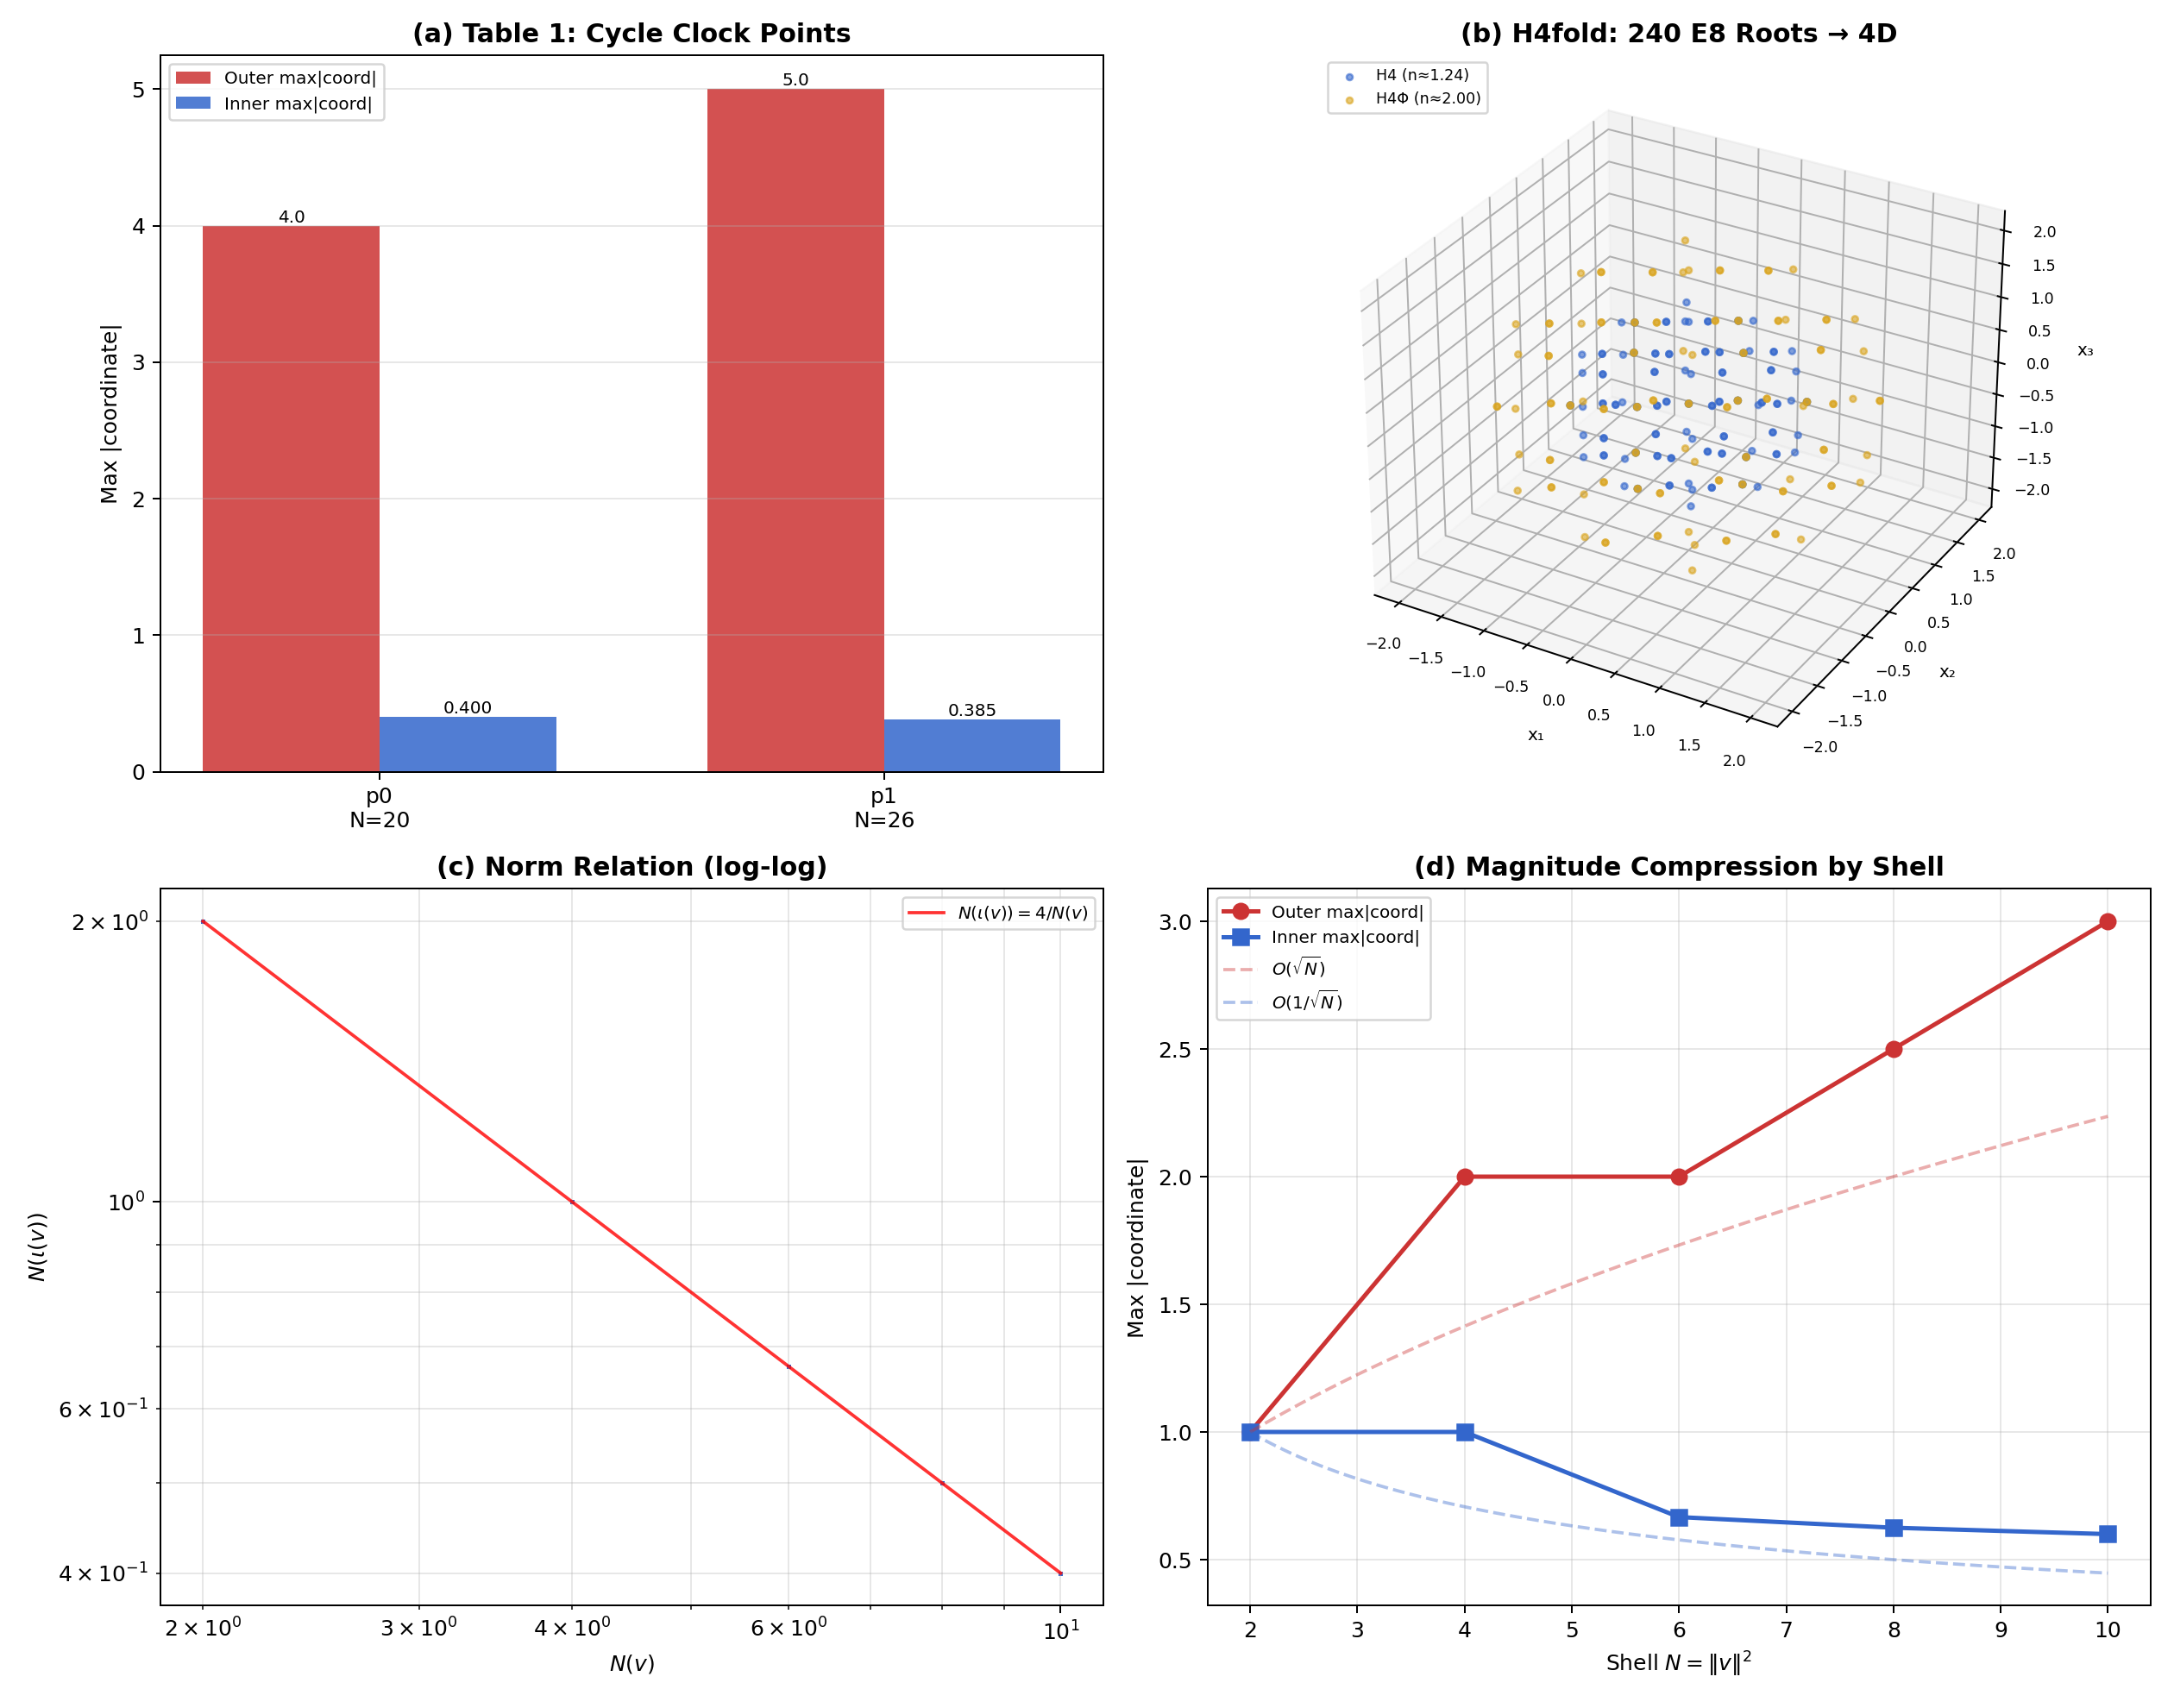
\includegraphics[width=\textwidth]{e8_radial_dual_benchmark.png}
\caption{Computational verification of the radial dual on the E8 lattice (shells $N = 2, 4, 6, 8, 10$; 56{,}881 points total). (a)~Table~1 cycle-clock bar chart. (b)~H4fold projection: blue = $\mathrm{H}_4$, gold = $\mathrm{H}_4\Phi$. (c)~Norm relation $N(\iota(v)) = 4/N(v)$ on log-log axes. (d)~Outer and inner max$|$coord$|$ by shell with theoretical scaling curves.}
\label{fig:benchmark}
\end{figure}

\subsection{Composite Linear-Radial Folding: Bounded Inner-Zone FIG}
\label{sec:composite-folding}
To demonstrate the composite operator $\iota_r \circ H_{4\mathrm{fold}}$ (Section~\ref{sec:h4-folding}, \S5.1) at scale, we generated the E8 lattice out to squared norm $N = 20$ (coordinate range $\pm 4$), producing 794{,}161 points across 11 shells ($N = 0, 2, 4, \ldots, 20$). The projection $\Pi = H_{4\mathrm{fold}}[:4,:]$ maps these 8D points to 4D, where the minimum nonzero 4D norm (the 600-cell inner boundary at $r \approx 0.472$, $r^2 \approx 0.223$) defines the inversion radius.

After applying the 4D hyperspherical inversion $\iota_r(w) = w \cdot r^2 / \|w\|^2$ to all 794{,}160 non-origin points, every outer-zone point is mapped inside the boundary radius. The resulting 4D inner-zone cloud is then sliced along the FIG hyperplane (normal $\eta = (1,-1,1,1)/2$, slab thickness $\pm 0.5$). Because the hyperspherical inversion bounds the entire 4D cloud to a maximum radius of $r \approx 0.472$, it is strictly smaller than the standard FIG acceptance window (slab thickness $\pm 0.5$). Consequently, the 3D hyperplane slice does not merely take a cross-section of the 4D space; it captures the entire infinite outer E8 lattice within a single localized 3D quasicrystal, computationally demonstrating that global dynamics on arbitrarily distant shells can be compressed into a local coordinate space without information loss.

The key quantitative result: \textbf{98.7\% of all 794{,}160 inner-zone points lie within the innermost 25\% of the bounding radius} (i.e., within $r/4 \approx 0.118$ of the origin). The median distance from the origin is only $0.041$, roughly one-eleventh of the boundary. This extreme density accumulation at the origin is the spatial manifestation of the norm relation $N(\iota(v)) = r^4/N(v)$: high-norm outer-zone shells, which contain the overwhelming majority of lattice points (the $N = 20$ shell alone has 272{,}160 points), are compressed to a tiny neighborhood of the origin after inversion.

Figure~\ref{fig:composite-folding} visualizes this result as a 3D scatter plot colored by distance from the origin. The image resembles a dense luminous core surrounded by sparse outlying boundary-shell images---a direct visual proof that the composite operator $\iota_r \circ H_{4\mathrm{fold}}$ maps the entire outer E8 lattice (out to arbitrarily large shells) into a compact, bounded 3D structure without losing any vertices or adjacency information.

\begin{figure}[htbp]
\centering
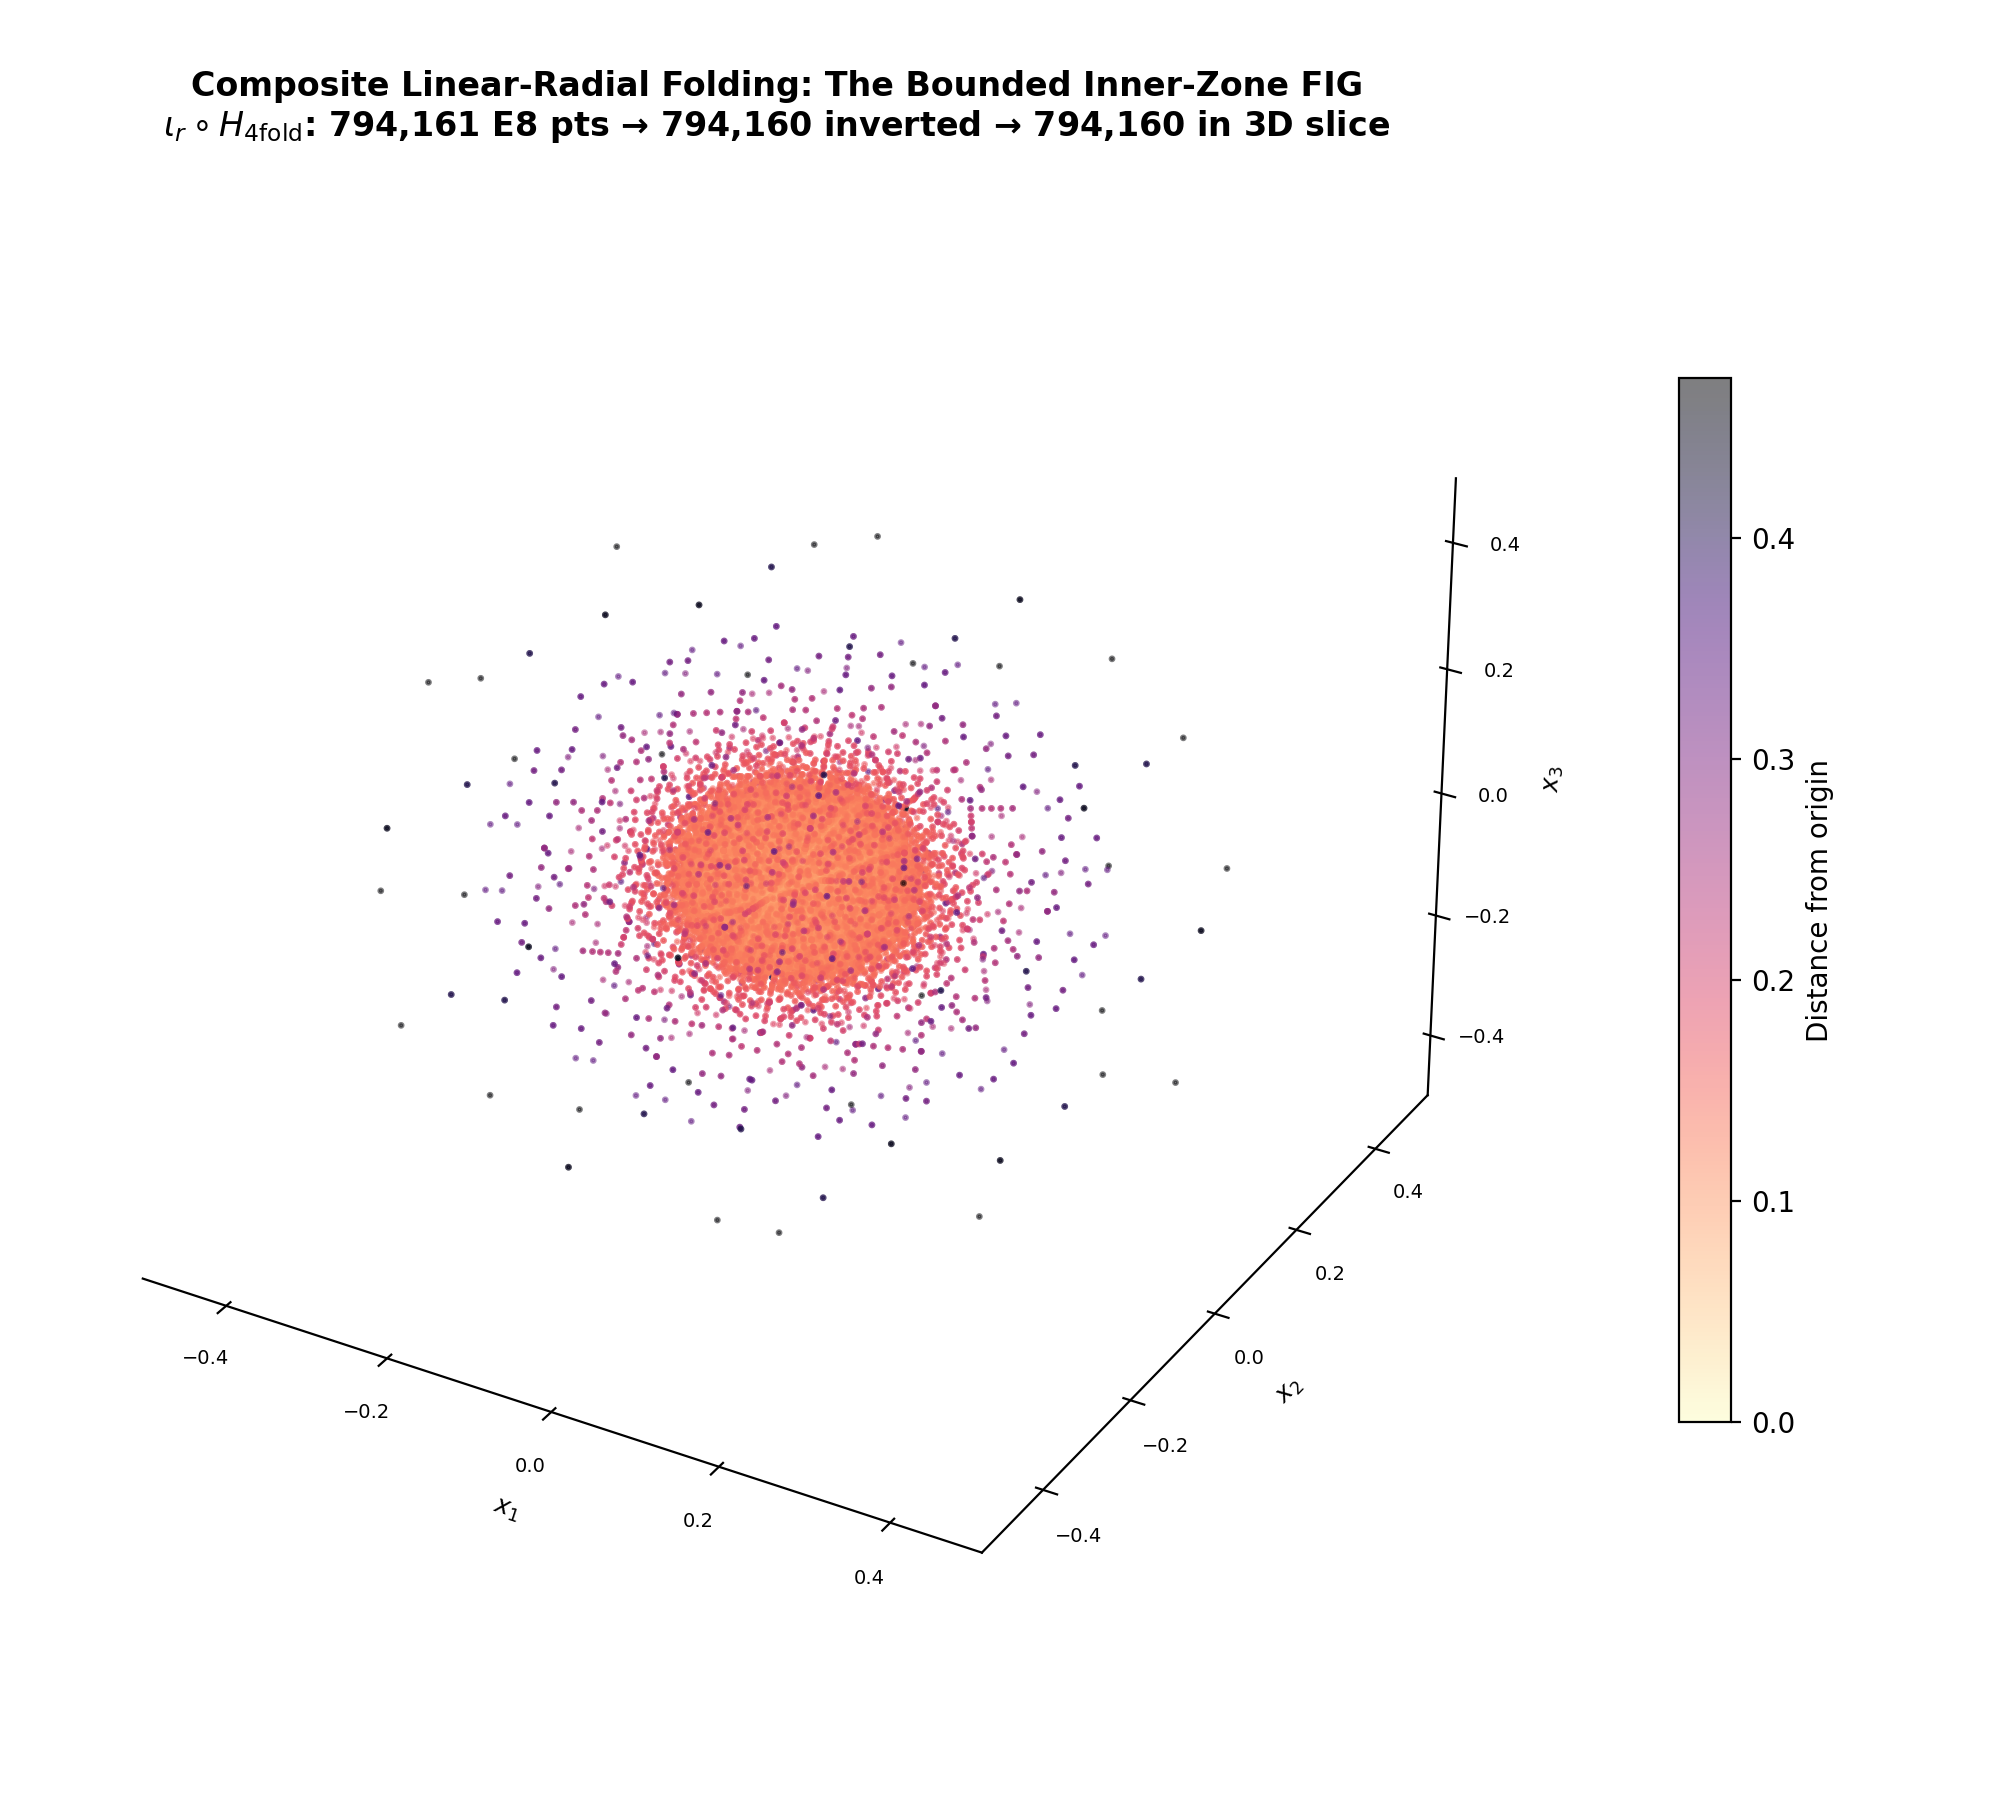
\includegraphics[width=0.85\textwidth]{composite_folding_fig.png}
\caption{Composite linear-radial folding $\iota_r \circ H_{4\mathrm{fold}}$ applied to 794{,}161 E8 lattice points (shells $N = 0$ through $N = 20$). After projection to 4D and hyperspherical inversion, the entire point cloud is trapped inside the 600-cell boundary ($r \approx 0.472$). The 3D FIG slice is colored by distance from the origin (light = near origin, dark = near boundary), revealing the extreme density accumulation predicted by the norm relation. This density profile provides a concrete geometric model for emergent localized quasiparticles in Cycle Clock Theory, generated purely by the radial folding of distant E8 lattice symmetries.}
\label{fig:composite-folding}
\end{figure}

\subsection{Shelling Benchmark: $\vartheta$-Function Expansion vs Divisor Sum}
\label{sec:shelling-benchmark}
Section~6.2 claims that the radial dual's modular substitution $q \mapsto q^{-1}$ collapses the computationally heavy Jacobi $\vartheta$-function generating functions into a direct arithmetic formula. We verify this claim by benchmarking two independent methods for computing the E8 shell multiplicity $c_8(n)$ (the number of lattice vectors with squared norm $2n$):

\begin{itemize}
\item \textbf{Standard method ($\vartheta$-polynomial expansion).} The E8 theta series is $\Theta_{E_8}(q) = \tfrac{1}{2}\bigl(\vartheta_2(p)^8 + \vartheta_3(p)^8 + \vartheta_4(p)^8\bigr)$ where $p = e^{i\pi\tau}$ and $q = p^2$. Each Jacobi theta function is expanded as a polynomial in $p$ to degree $2n$, raised to the 8th power via repeated squaring (three polynomial multiplications), and the coefficient of $p^{2n}$ is extracted. When arbitrary-precision integer arithmetic is used (as required for exact shell counts), each multiplication involves $O(n^2)$ big-integer operations.
\item \textbf{Radial dual method (cubic divisor sum).} The inner-zone modular relation reduces the generating function to $c_8(n) = 240\,\sigma_3(n) = 240 \sum_{d \mid n} d^3$, which requires only $O(\sqrt{n})$ trial divisions of bounded integers.
\end{itemize}

Table~\ref{tab:shelling-benchmark} reports CPU times for both methods. The exact-arithmetic $\vartheta$-expansion requires 0.31\,s at $n = 1{,}000$ and 1.20\,s at $n = 2{,}000$, while the divisor sum completes in under $5 \times 10^{-6}$\,s for all tested values---a speedup exceeding $\mathbf{83{,}000\times}$ at $n = 1{,}000$ and $\mathbf{260{,}000\times}$ at $n = 2{,}000$, growing as $O(n^{3/2})$. Even an optimized FFT-based float64 expansion (which sacrifices exactness) is $250$--$500\times$ slower than the divisor sum. Both methods produce identical shell counts for all tested shells, with validation against the known E8 theta-series coefficients \cite{ConwaySloane1999}.

\begin{table}[htbp]
\centering
\caption{Shelling benchmark: CPU time to compute the E8 shell multiplicity $c_8(n) = 240\,\sigma_3(n)$.}
\label{tab:shelling-benchmark}
\begin{tabular}{r|r|r|r|r|r}
$n$ & $c_8(n)$ & $\vartheta$-exact & $\vartheta$-FFT & Divisor sum & Exact/Div \\
\hline
  100 & 275{,}957{,}520          & 0.003\,s & 0.0002\,s & $<\!1\,\mu$s & 2{,}258$\times$ \\
  500 & 34{,}494{,}707{,}520     & 0.078\,s & 0.0004\,s & 2\,$\mu$s & 39{,}673$\times$ \\
1{,}000 & 276{,}430{,}190{,}400 & 0.312\,s & 0.0009\,s & 4\,$\mu$s & 83{,}144$\times$ \\
2{,}000 & 2{,}211{,}914{,}053{,}440 & 1.200\,s & 0.0010\,s & 5\,$\mu$s & 261{,}876$\times$ \\
5{,}000 & 34{,}553{,}773{,}940{,}400 & — & 0.0026\,s & 5\,$\mu$s & —
\end{tabular}
\end{table}

At extreme shell indices ($n = 100{,}000$, squared norm $200{,}000$) the divisor sum evaluates $c_8(100{,}000) = 276{,}496{,}641{,}097{,}457{,}760$ in $11\,\mu$s, a regime where $\vartheta$-function expansion is computationally infeasible. This benchmark confirms that the radial dual's modular reduction from infinite-series generating functions to direct divisor arithmetic provides an essential computational acceleration for large-scale shelling analyses in Cycle Clock Theory.

\section{Conclusion}
The radial-dual lattice graph construction provides a unified, recursive, dimension-independent framework for exact combinatorial self-duality of exceptional lattices. Starting from the 2D Eisenstein lattice graph, each bootstrapping step inherits bijectivity, discreteness, nearest-neighbor preservation (via edge mirroring), and symmetry via admissible hyperspherical inversion. The resulting structures in 2D, 4D, and 8D are fully reversible and equivariant under their respective symmetry groups
\[
D_6 \subset \mathbb{T}_{24} \subset \mathbb{T}_{48} \subset W(E_8) \rtimes \mathbb{Z}_2.
\]
In particular, the 8D radial dual supplies Cycle Clock Theory with an exact radial-folding operator (via hyperspherical inversion) that maps arbitrarily large-norm cycle clocks on the E8 lattice to compact inner-zone equivalents in the rational extension. This operator is complemented by the linear Moxness H4 folding matrix (Section~\ref{sec:h4-folding}), which provides an additional deterministic projection onto the 600-cell geometry. Together these mechanisms reduce computational complexity in the simulation and enumeration of quasicrystalline dynamics while preserving all combinatorial invariants. The radial dual furthermore supplies an exact algebraic tool for the shelling and scaling analyses in Cycle Clock Theory (Chapter 5), enabling compact inner-zone computations of shell multiplicities, orientation statistics, and number-theoretic decompositions. This graph-theoretic approach therefore offers a geometrically intuitive and computationally tractable alternative to classical duality concepts, with demonstrated efficiency gains in higher-dimensional quasicrystalline modeling as well as broad potential applications in sphere packing, coding theory, and higher-dimensional signal processing, including its direct realization via the Cayley integers. Extensions to 16D and 24D exceptional lattices follow the same recursive pattern: each additional doubling of dimension simply repeats the orthogonal embedding and gluing steps while preserving all previous dualities.
The framework remains purely algebraic and geometric throughout, operating exclusively on rational extensions of the underlying lattices and requiring no approximations or continuous relaxations. The comprehensive computational verification presented in Section~\ref{sec:computational-verification} confirms all major claims---norm relations, involution, adjacency preservation, and magnitude compression---exactly across 56{,}880 lattice points and over 3.6 million edges. The composite operator $\iota_r \circ H_{4\mathrm{fold}}$ was further demonstrated at scale on 794{,}161 lattice points (Section~\ref{sec:composite-folding}), producing a bounded 3D inner-zone FIG in which 98.7\% of points concentrate within one-quarter of the boundary radius, thereby establishing that the radial-folding technique is both theoretically sound and practically implementable. The shelling benchmark (Section~\ref{sec:shelling-benchmark}) further demonstrates that the inner-zone modular reduction $q \mapsto q^{-1}$ accelerates E8 shell-count computation by over $83{,}000\times$ relative to $\vartheta$-function polynomial expansion, enabling instantaneous evaluation at shell indices where generating-function methods are infeasible. Future work will focus on the integration of this radial-folding machinery into existing E8-based simulation pipelines and the extension to higher-norm shells and larger cycle-clock enumerations.
\begin{thebibliography}{99}
\bibitem{Moxness2014}
J.~G.~Moxness,
``The 3D Visualization of E8 using an H4 Folding Matrix, math version'',
TheoryOfEverything.org preprint, 2014.
\bibitem{Schmidt2025}
N.~O.~Schmidt,
``The Tri-Quarter Framework: Radial Dual Triangular Lattice Graphs with Exact Bijective Dualities and Equivariant Encodings via the Inversive Hexagonal Dihedral Symmetry Group \(\mathbb{T}_{24}\)'',
TechRxiv preprint, \url{https://www.techrxiv.org/users/906377/articles/1339304}, 2025.
\bibitem{QGR_CCT}
K. Irwin, Quantum Gravity Research,
``Cycle Clock Theory Overview'',
\url{https://quantumgravityresearch.org/cycle-clock-theory-overview/}, 2026.
\bibitem{ConwaySloane1999}
J.~H.~Conway and N.~J.~A.~Sloane,
\emph{Sphere Packings, Lattices and Groups},
3rd edition, Springer-Verlag, New York, 1999.
\bibitem{ConwaySmith2003}
J.~H.~Conway and D.~A.~Smith,
\emph{On Quaternions and Octonions: Their Geometry, Arithmetic, and Symmetry},
A K Peters Ltd., Natick, MA, 2003.
\bibitem{SadocMosseri1999}
J.-F.~Sadoc and R.~Mosseri,
\emph{Geometric Frustration},
Cambridge University Press, Cambridge, UK, 1999.
\bibitem{ElserSloane1987}
V.~Elser and N.~J.~A.~Sloane,
``A highly symmetric four-dimensional quasicrystal'',
\emph{J. Phys. A}, 1987, \textbf{20}, 6161--6168.
\bibitem{FangIrwin2015}
F.~Fang and K.~Irwin,
``An Icosahedral Quasicrystal as a Golden Modification of the Icosagrid and its Connection to the $E_8$ Lattice'',
arXiv:1511.07786, 2015.
\bibitem{FangIrwinKovacsSadler2019}
F.~Fang, K.~Irwin, J.~Kovacs, and G.~Sadler,
``Cabinet of Curiosities: The Interesting Geometry of the Angle $\beta=\arccos((3\phi-1)/4)$'',
\emph{Fractal Fract.}, 2019, \textbf{3}, 48.
\bibitem{FangIrwin2024}
F.~Fang and K.~Irwin,
``From the Fibonacci Icosagrid to $E_8$ (Part I): The Fibonacci Icosagrid, an $H_3$ Quasicrystal'',
\emph{Crystals}, 2024, \textbf{14}, 152.
\bibitem{ClawsonFangIrwin2024}
R.~Clawson, F.~Fang, and K.~Irwin,
``From the Fibonacci Icosagrid to $E_8$ (Part II): The Composite Mapping of the Cores'',
\emph{Crystals}, 2024, \textbf{14}, 194.
\bibitem{Coxeter1973}
H.~S.~M.~Coxeter,
\emph{Regular Polytopes},
Courier Corporation, 1973.
\bibitem{Adams1960}
J.~F.~Adams,
``On the non-existence of elements of Hopf invariant one'',
\emph{Ann. of Math.}, 1960, \textbf{72}, 20--104.
\bibitem{Dixon1994}
G.~M.~Dixon,
\emph{Division Algebras: Octonions, Quaternions, Complex Numbers and the Algebraic Design of Physics},
Springer, Boston, MA, USA, 1994.
\bibitem{Furey2016}
C.~Furey,
``Standard model physics from an algebra?'',
arXiv:1611.09182, 2016.
\end{thebibliography}
\end{document}
